\add{Bugfixing in tex code}
\chapter{Grundlagen}
\label{grundlagen}
\add{Correction}
\add{urls in footnotes}
\noindent In diesem Kapitel werden die theoretischen Grundlagen von essentiellen Komponenten dieser Arbeit erläutert. Dazu wird die Relevanz von Entwurfsmustern erklärt und auf zwei bedeutende Muster näher eingegangen. Diese sind sowohl erforderlich für die folgenden Kapitel als auch für das Verständnis der softwaretechnischen Prinzipien von JavaFX.\\
Danach wird die JavaFX-Bibliothek vorgestellt und fundamentale Konzepte wie beispielsweise die auf der \ac{xml} basierende Layouting-Sprache erläutert.\\
Abschließend wird das generelle Annotationenkonzept in der Informatik mit speziellen Fokus auf die Programmiersprache Java erklärt. Dabei werden die verschiedenen Annotationstypen näher beschrieben und die Möglichkeiten der eigentlichen Auswertung dieser skizziert. Komplexe Konzepte werden dabei durch visuelle Beispiele wie Quelltextausschnitte\footnote{Die dargestellten Quelltextausschnitte sind aufgrund der Simplizität nicht immer kompilierbar, da irrelevante Programmkonstrukte wie Importe von Klassen nicht für ein Verständnis des dargestellten Kontextes benötigt werden.} oder \ac{uml}-Klassendiagramme untermauert und möglicherweise vereinfacht. 

\section{Entwurfsmuster}
\label{entwurfsmuster}
Entwurfsmuster sind Lösungen für immer wieder auftretende Probleme bei der Softwareentwicklung. Sie stellen eine wiederverwendbare Problemlösung für architektonisch begründete Problematiken dar, welche im Endeffekt durch nur wenige Klassen und Schnittstellen effektiv und schnell gelöst werden können. Ein Entwurfsmuster setzt sich aus vier Komponenten zusammen: Dem Namen des Musters, dem zu lösenden Problem, der daraus resultierende Lösung und die auftretenden positiven sowie negativen Auswirkungen bei Nutzung des Musters \cite{Gamma1993}.\\
Im Folgenden werden das \ac{mvc}- sowie das Beobachter-Entwurfsmuster für das Verständnis von JavaFX Prinzipien beschrieben.
\subsection{Beobachter}
Das Beobachter Entwurfsmuster ist ein essentieller Bestandteil von vielen auf der reaktiven Programmierung aufbauenden Bibliotheken und APIs \cite{Salvaneschi2015} und obwohl es häufig in der Kritik steht, wird es dennoch in vielen Bereitstellungsumgebungen genutzt \cite{Maier2010}.
\begin{figure}[H]
	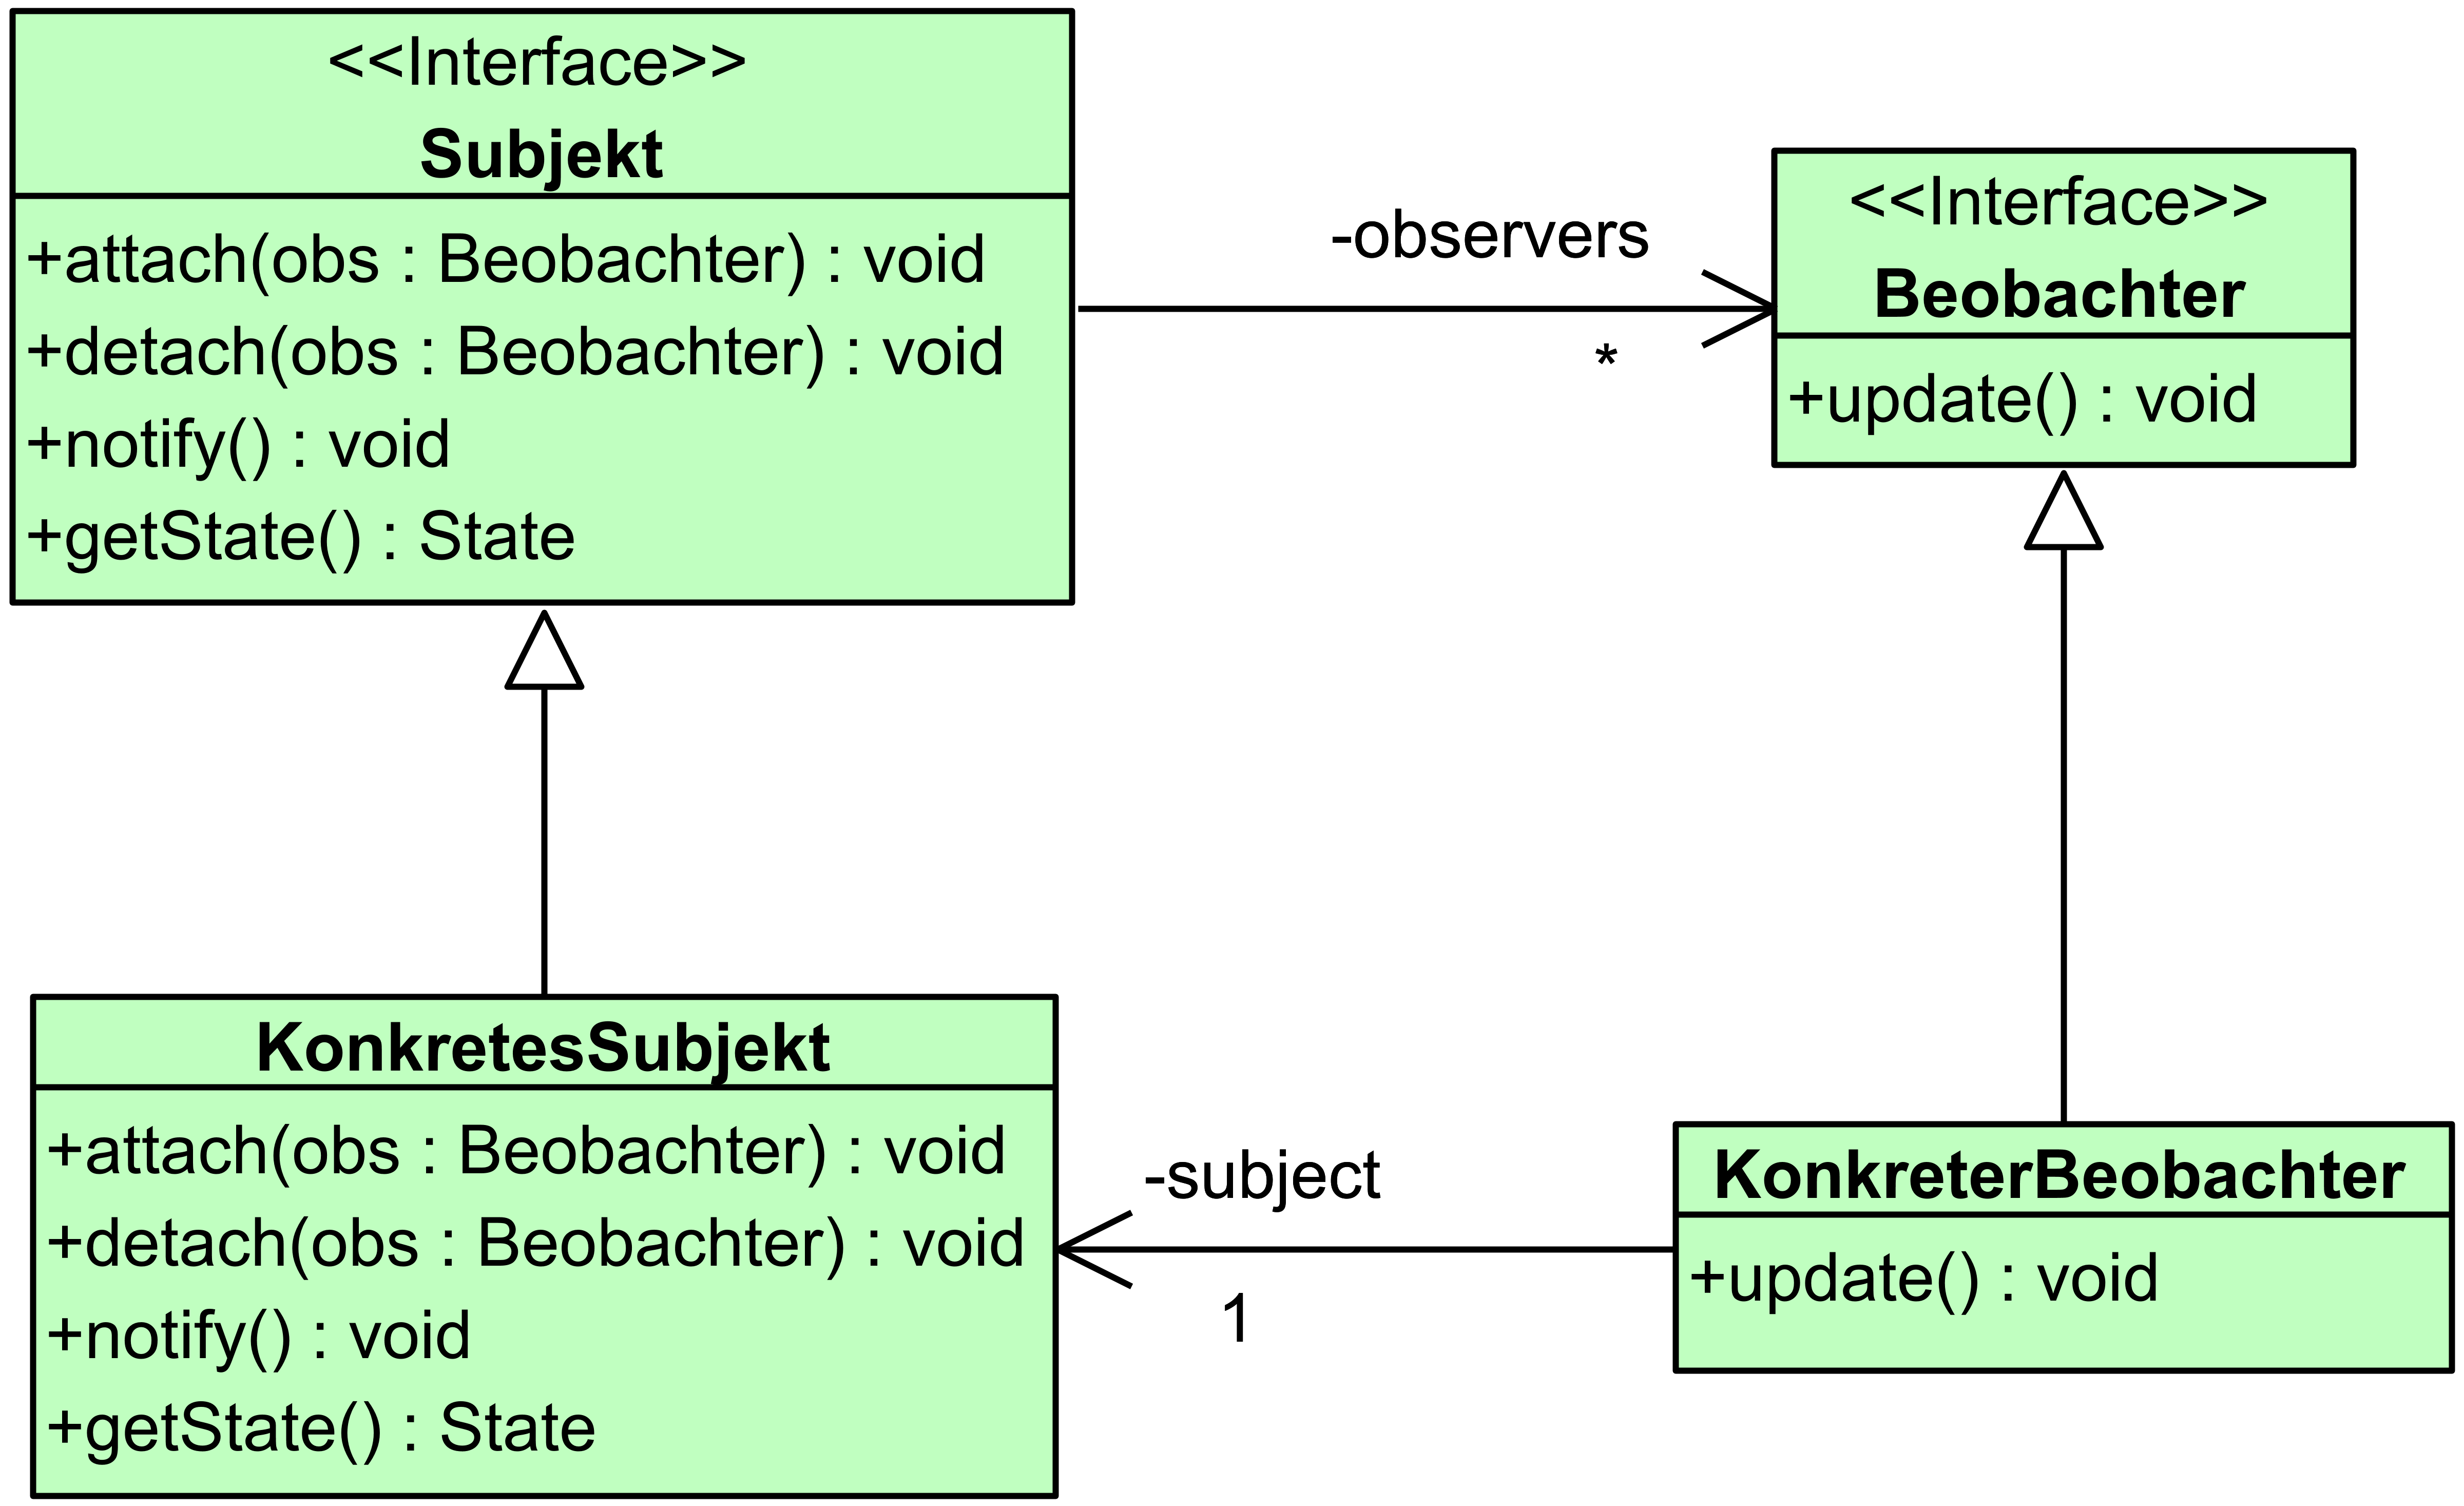
\includegraphics[width=\textwidth]{Abbildungen/Observer Pattern.png}
	\caption{UML-Diagramm -- Beobachter-Entwurfsmuster}
	\label{fig:observer_pattern}
\end{figure}
\noindent Das Entwurfsmuster benötigt für die korrekte Implementierung mindestens vier Komponenten (siehe \autoref{fig:observer_pattern}) \cite{Gamma1993}:
\begin{description}
	\item Das \texttt{\textbf{Subjekt}}, ist das zu beobachtende Objekt, welches zu jedem Zeitpunkt alle seine Beobachter in einer internen Datenstruktur speichert. Es besitzt Methoden zum An- und Abmelden von Beobachtern und ist in der Lage alle Beobachter bei eventuellen Zustandsänderungen zu benachrichtigen.
	\item Der \texttt{\textbf{Beobachter}} bietet eine Schnittstelle für Objekte, welche bei einer Zustandsänderung des Subjekts informiert werden sollen.
	\item Die \texttt{\textbf{KonkretesSubjekt}} Komponente ist die konkrete Implementierung der Subjekt Schnittstelle und ist fähig, einen internen Zustand zu verwalten, sowie bei einer Änderung von diesem, alle registrierten Beobachter zu informieren.
	\item Ein \texttt{\textbf{KonkreterBeobachter}} besitzt eine Referenz auf das zu beobachtende Subjekt und seinen internen Zustand. Bei einer Aktualisierung des Subjektzustands, wird auch der interne Zustand des konkreten Beobachters aktualisiert.
\end{description}
\newpage
\subsection{MVC}
Das \ac{mvc} Entwurfsmuster\footnote{Je nach Interpretation, kann es sich bei dem \ac{mvc} Muster auch um ein Architekturmuster handeln, bei welchem Model, View und Controller als Schichten einer Architektur gesehen werden und nicht direkt als beispielsweise Klassen implementiert werden.} ist ein de facto Standard der objektorientierten Programmierung \cite{Deacon1995}, welches für eine Trennung von grafischer Oberfläche, Eingaben des Benutzers und dem eigentlichen Anwendungsmodell sorgt \cite{Burbeck1992}. Hält eine Anwendung diese strikte Trennung ein, so genügt sie dem softwaretechnischen \ac{soc} Prinzip \cite{Grant2014}, woraus wiederum der Wartungsprozess vereinfacht und die Testbarkeit erhöht wird.
\begin{figure}[H]
	\centering
	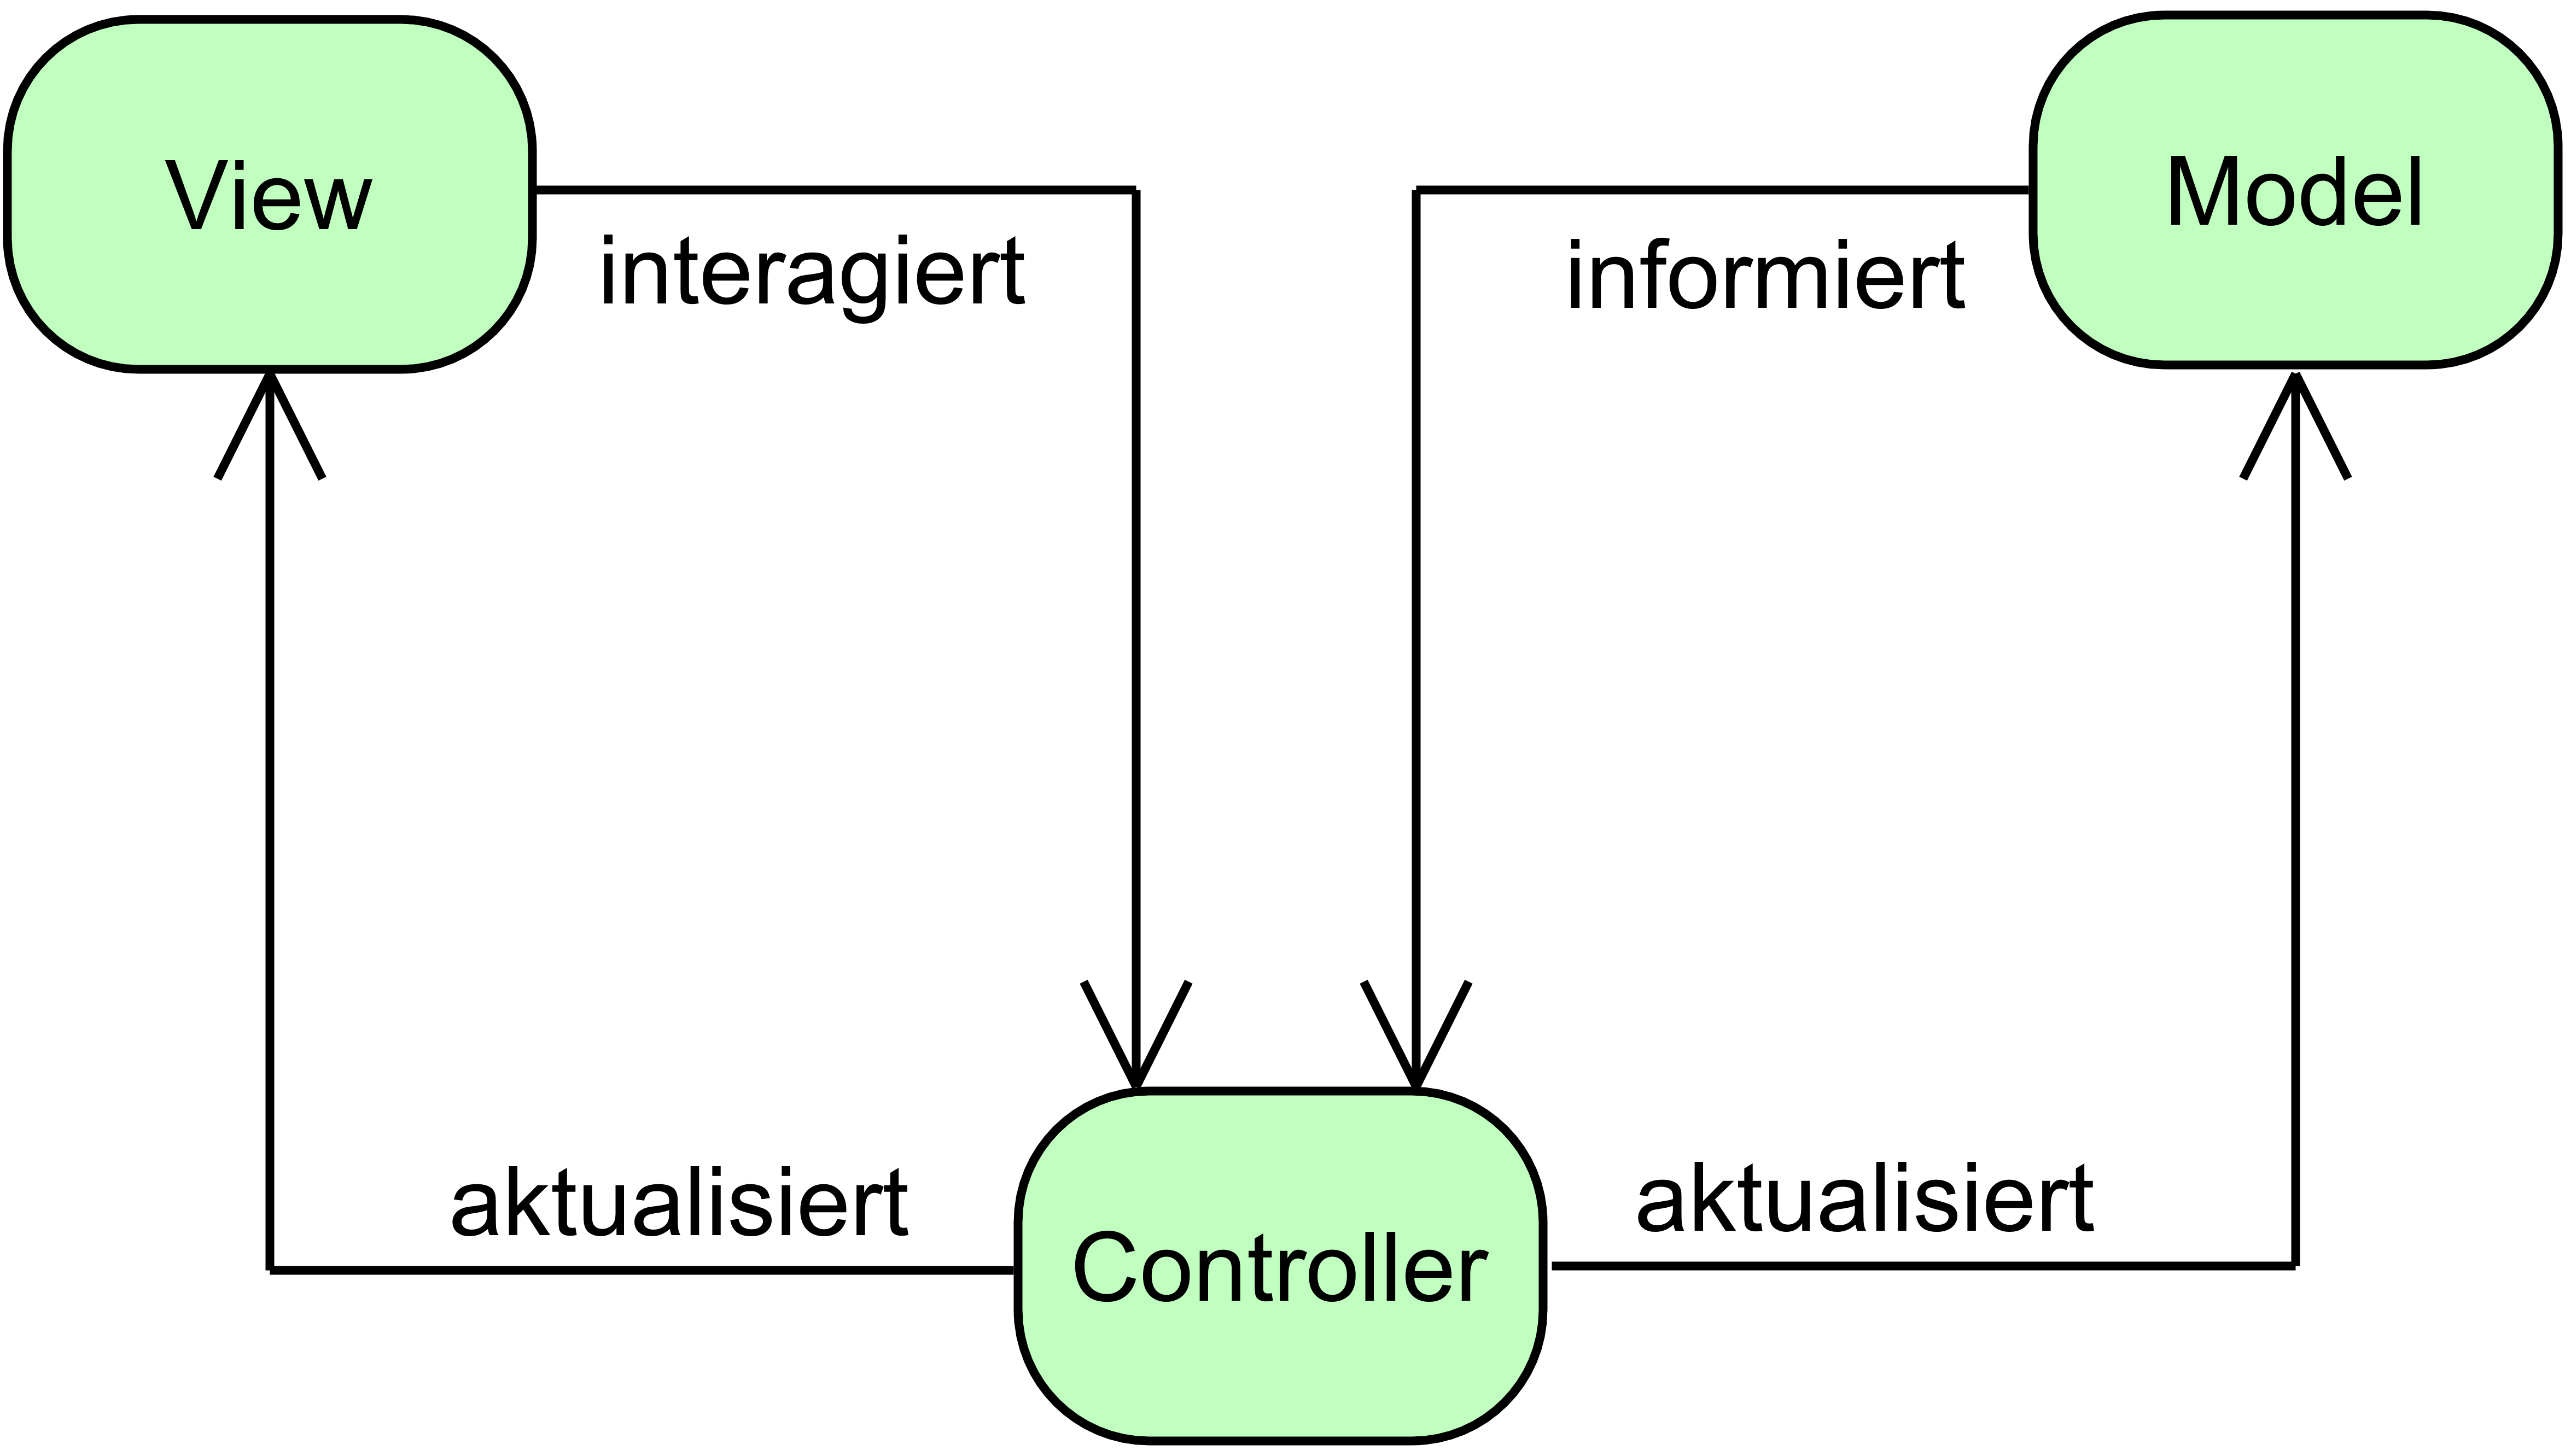
\includegraphics[width=\textwidth-2cm]{Abbildungen/MVC Pattern.png}
	\caption[Diagramm -- MVC-Entwurfsmuster]{Diagramm -- MVC-Entwurfsmuster: Die blauen Pfeile stellen indirekte Beziehungen dar, welche meist durch die Nutzung eines Eventsystems auf Basis des Beobachter Musters implementiert werden.}
	\label{fig:mvc_pattern}
\end{figure}
\noindent Die vom \ac{mvc} Muster klassische Struktur\footnote{In der Literatur sind viele Interpretationen des \ac{mvc} Musters beschrieben. Eine strikte Unterteilung der drei Komponenten ist jedoch immer vorhanden.} ist, wie in \autoref{fig:mvc_pattern} zu sehen, in drei Komponenten unterteilt \cite{Deacon1995}:
\begin{description}
	\item Das \texttt{\textbf{Model}} beinhaltet alle Klassen welche für die Logik und die Datenhaltung der Anwendung verantwortlich sind und ist vollständig unabhängig vom View.
	\item Der \texttt{\textbf{View}} stellt die Anwendung dar, ermöglicht eine Interaktion mit diesem und ist in den meisten Applikationen äquivalent zu einer grafischen Benutzeroberfläche.
	\item Der \texttt{\textbf{Controller}} ist für das Verändern des Views verantwortlich. So werden beispielsweise Interaktionen mit der Benutzeroberfläche wie ein Schaltflächenklick im Controller verarbeitet, was wiederum den View aktualisiert. Der View und das Model sind vollständig entkoppelt und der Controller ist die Schnittstelle zwischen diesen.
\end{description}
\section{JavaFX}
\label{javafx}
\noindent JavaFX ist eine auf Java basierte, quelloffene Bibliothek für das Entwickeln von grafischen Benutzerschnittstellen für Client Applikationen. Im Vergleich zum Vorgänger GUI-Toolkit Java-Swing, bietet JavaFX ein modernes, zeitgemäßes Design der allgemeinen Benutzeroberfläche sowie den dort enthaltenen Schaltflächen und Komponenten \cite{Sharan2015}. Kombiniert mit den objektorientierten Konzepten von Java, ist JavaFX in der Lage auch komplexe nebenläufige Anwendungen mit vielen Abhängigkeiten darzustellen und aufgrund der Plattformunabhängigkeit auch ohne viele Restriktionen in allen bekannten Betriebssystemen einsetzbar.\\
Dazu ist JavaFX auch weitgehend konform mit bekannten Entwurfsmustern der Softwareentwicklung wie beispielsweise dem \ac{mvc}\footnote{Die Beschreibung des \ac{mvc} Musters aus \autoref{fig:mvc_pattern} ist nicht vollständig auf die JavaFX Situation anzuwenden, da der  \texttt{View} meistens in eine FXML-Datei ausgelagert wird und deshalb nicht unbedingt mit dem \texttt{Model} interagiert.}- oder dem Beobachter-Muster, weshalb implementierte Anwendung selbst bei vielen \ac{loc}, eine grundsätzlich hohe Strukturiertheit auf Quelltextebene aufweisen. Durch die Verwendung von Properties und Bindings (siehe \autoref{properties_und_bindings}) ist es auch möglich das \ac{mvvp} Muster zu nutzen. Das grafische Layout kann dabei nicht ausschließlich durch Java-Quelltext sondern auch mittels der an die \ac{xml} angelehnte Markup-Sprache FXML erstellt werden. Letzteres kann durch externe Tools wie dem Scene-Builder enorm vereinfacht werden \cite{Vos2018}.

\subsection{Aufbau und Szenengraph}
\label{javafx_szenengraph}
Damit eine JavaFX-Anwendung als solche identifiziert werden kann, muss die Hauptklasse von der \texttt{Application}-Klasse erben. Die Namensgebung der Klassen, welche für die Struktur bzw. den Aufbau einer JavaFX-Anwendung zuständig sind, basiert auf Begriffe der Theaterumgebung \cite{Anderson2019}:
\begin{description}
	\item Die \textbf{\texttt{Stage}} Klasse repräsentiert ein Anwendungsfenster, welches das Design des Fensterlayouts des aktuell genutzten Betriebssystems nutzt. Eine \texttt{Stage} ist teilweise modifizierbar, so können beispielsweise die Standardschaltflächen in der Titelleiste entfernt oder deaktiviert werden. Werden mehrere Fenster benötigt, so können nach dem Initialisieren der Haupt-\texttt{Stage} durch die JavaFX-Plattform, manuell weitere hinzugefügt werden.
	\item Die \textbf{\texttt{Scene}} Klasse ist für das Layout und die Darstellung von vorhandenen oder selbsterstellten JavaFX-Komponenten verantwortlich. Jede Komponente, welche durch eine \texttt{Scene}-Instanz angezeigt und verwaltet werden soll, wird in einer hierarchisch angeordneten, objektorientierten Datenstruktur eingefügt, welche in der Computergrafik als Szenengraph bekannt ist \cite{Hughes2013}. Jeder \texttt{Stage} muss zwangsläufig eine \texttt{Scene} zugewiesen werden.
	\item Die \textbf{\texttt{Node}} Klasse ist eine darstellbare Komponente im Szenengraphen wie beispielsweise eine Schaltfläche oder ein Containerelement. \texttt{Node} Instanzen im Szenengraph können Kindelemente enthalten und maximal einem Elternelement zugeordnet sein. Der Szenengraph ähnelt somit einer Baumstruktur mit einer Wurzel und einem oder mehreren Blättern. Damit eine \texttt{Node}-Instanz Kindelemente besitzen darf, muss diese immer von der abstrakten \texttt{Parent}-Klasse erben. Das Layouting und die Positionierung im lokalen Koordinatensystem wird bei vorhandenen Kindelementen immer durch das Elternelement kontrolliert. Jede darzustellende Komponente muss von der \texttt{Node}-Klasse erben \cite{Juneau2013}.
\end{description}
Ein minimales Beispiel für eine voll funktionsfähige JavaFX-Anwendung, welche das Zusammenspiel der oben genannten Konzepte und Klassen widerspiegelt, ist in \autoref{lst:example_javafxapp} dargestellt.\\
\begin{figure}[H]
	\begin{lstlisting}[caption={Beispiel -- Minimale JavaFX-Anwendung.}, captionpos=b, label=lst:example_javafxapp]
		public class TestApplication extends Application {
			
			public static void main(String[] args) {
				Application.(@\tikzmark{entryLeft}{}@)launch(args)(@\tikzmark{entryRight}{}@);
			}
			
			@Override
			public void start(Stage primaryStage) {
				final Pane root = new Pane();
				root.getChildren().add(new Button("TestButton"));
				final Scene scene = new Scene(root, 250, 250);
				primaryStage.setScene(scene);
				primaryStage.show();
			}
		(@
		\begin{tikzpicture}[overlay,remember picture]
			\renewcommand{\VerticalShiftForBar}{0em, -1.5ex}
			\renewcommand{\Stub}{0em, 0.6ex}
			\DrawOverBar[-, red, thick]{entryLeft.north}{entryRight.north}
			\node[draw] (entrypoint) at (8.3, 4.3) {Einstiegspunkt};
			\renewcommand{\VerticalShiftForArrows}{0, -1ex}
			\DrawArrow[red, in=180, out=-45]{entry}{entrypoint}{-4.55em, 0}
			\Circled{1}{0.45, 2.4}
			\Circled{2}{0.45, 1.35}
		\end{tikzpicture}
		@)
		}
	\end{lstlisting}
	Nach der Initialisierung der JavaFX Anwendung wird in \CircledStandalone{1} das Wurzelelement des Szenengraphen erstellt und um eine \texttt{Button} Instanz erweitert. Dieses wird dann in \CircledStandalone{2} zu einem \texttt{Scene} Objekt hinzugefügt, welche wiederum als Szene der \texttt{primaryStage} dient. Das Beispiel wird mit dem Anzeigen der Stage beendet.
\end{figure}
\subsection{Properties und Bindings}
\label{properties_und_bindings}
JavaFX besitzt eine auf dem JavaBeans-System und dem Observer-Entwurfsmuster basierende API, welche es dem Programmierer ermöglicht, eine synchronisierende Beziehung zwischen zwei oder mehr Variablen zu erstellen. Wird eine Variable in einer solchen Beziehung geändert, so wird automatisch auch die andere geändert \cite{Hommel2013}. Dabei ist es auch möglich, Event Listener für eigene oder durch von JavaFX-Nodes automatisch erzeugte Properties zu registrieren. Soll beispielsweise Quelltext ausgeführt werden, wenn eine Änderung eines Wertes einer Property festgestellt wird, so kann dies mit dem Erstellen einer \texttt{ChangeListener}-Instanz durchgeführt werden \cite{Gao2019}. 
\begin{figure}
	\begin{lstlisting}[caption=Beispiel -- ChangeListener \& EventHandler., captionpos=b, label=lst:property_example]
	Button btn = new Button("Test");
	// ChangeListener für den Schaltflächentext
	btn.textProperty().addListener((obs, oVal, nVal) -> {
		System.out.println(nVal);
	});	
	// EventHandler für die Schaltflächenaktivierung
	btn.setOnAction(e -> {
		System.out.println("Clicked!");
	})
	\end{lstlisting}
\end{figure}
\noindent Im ersten Teil von \autoref{lst:property_example} soll der Text einer Schaltfläche bei einer Änderung auf die Konsole ausgegeben werden. Dazu wird mittels Lambda Ausdruck ein neuer \texttt{ChangeListener} mit der \texttt{StringProperty} der Schaltfläche verknüpft.\\
Des Weiteren unterstützt JavaFX ein Event-System, welches anhand von verschiedenen Aktionen Events durch den Szenengraphen propagiert. Ein solches Event wird beispielsweise durch das Eintragen von Text in ein Textfeld oder das Aktivieren einer Dropdown-Liste ausgelöst. In zweiten Teil von \autoref{lst:property_example} wird ein \texttt{EventHandler} für das Aktivieren einer Schaltfläche erstellt.

\subsection{Layouting: FXML vs. Quelltext}
Wie in der Einleitung schon angedeutet, ist es möglich das Layout der Anwendung auch per FXML zu erstellen. Eine Prävention von Boilerplate-Code kann durch das Auslagern von häufig verwendeten JavaFX-Komponenten in externe FXML-Dateien erfolgen \cite{Kruk2018}. Das Verwenden von solchen Dateien sorgt für eine bessere Trennung von Controllern und Logik im Sinne des z.B. \ac{mvc}-Entwurfsmusters \cite{Juneau2013} und durch die hohe Konfigurierbarkeit sind für eine eventuelle Veröffentlichung der Applikation wichtige Konzepte wie die Internationalisierung, leichter umzusetzen \cite{Steyer2014}. Durch das Parsen und Aufbauen des Szenengraphen zur Laufzeit des Programms ist eine Verwendung von FXML-Dateien jedoch langsamer als benötigte Komponenten direkt im Java Quelltext zu deklarieren. Fast alle JavaFX-Nodes können ohne Weiteres in XML-Elementen verwendet und angepasst werden. Außerdem ist es möglich, direkt eine manuell erstellte Controller-Klasse mit einer FXML-Datei zu assoziieren. Das Laden einer FXML-Datei und das darauffolgende Aufbauen des Szenengraphen wird durch die \texttt{FXMLLoader}-Klasse durchgeführt. Das Layouting-Beispiel aus \autoref{lst:example_javafxapp} ist als eine funktionsgleiche FXML Variante in \autoref{lst:example_fxmllayouting} zu erkennen. Das Laden der Datei wird durch das Instanziieren eines neuen \texttt{FXMLLoader} Objekts, wie in \autoref{lst:example_fxmlloading} dargestellt, ermöglicht.
\noindent Um eine Controller-Klasse mit der FXML-Datei zu assozieren, kann das Wurzelelement dieser durch das \texttt{fx:controller} Attribut erweitert werden. Der Name des Controllers ist hierbei der voll qualifizierte Klassenname. Neben externen FXML-Dateien können auch externe \ac{css}-Dateien für das Design des Layouts verwendet werden. In \autoref{appendix:controllerbased_javafx_application} ist ein vollständig kompilierbares JavaFX-Programm welches aus einem Controller, einer FXML-Datei sowie einer CSS-Datei aufgebaut ist zu finden.

\begin{figure}[H]
	\begin{lstlisting}[caption={Beispiel -- FXML Layouting.}, captionpos=b, label=lst:example_fxmllayouting, language=XML]
	<?xml version="1.0" encoding="UTF-8"?>
	
	<?import javafx.scene.layout.Pane?>
	<?import javafx.scene.control.Button?>
	
	<Pane xmlns="http://javafx.com/javafx">
	<Button>TestButton</Button>
	</Pane>
	\end{lstlisting}
\end{figure}
\begin{figure}[H]
	\begin{lstlisting}[caption={Beispiel -- FXML Ladeprozess.}, captionpos=b, label=lst:example_fxmlloading]
	Pane load(String fxmlPath) throws IOException {
	return new FXMLLoader(getClass().getResource(fxmlPath)).load();
	}
	\end{lstlisting}
\end{figure}

\section{Java-Annotationen}
\label{java_annotationen}
\noindent Annotationen sind in der Sprachwissenschaft eine Möglichkeit einen vorhandenen Text mit Anmerkungen zu versehen für beispielsweise Disambiguierung, also das Eliminieren von Mehrdeutigkeiten eines Wortes oder für das Erklären von komplexen Textabschnitten. Sie geben dem Leser Zusatzinformationen um Sachverhalte einfacher darzustellen und sorgen dadurch für ein schnelleres bzw. besseres Verständnis des Textes. Dabei sind solche Anmerkungen kein Hauptbestandteil von Texten sondern dienen ausschließlich als Ergänzung.\\
In der Informatik sind Annotationen ebenfalls nur ein deskriptives Strukturkonzept, welche es dem Entwickler ermöglicht, verschiedenen strukturellen Elementen der Programmierung (wie Felder oder Klassen), Metadaten zuzuweisen \cite{Yu2019}. Das Nutzen von Annotationen in Anwendungen ist aufgrund ihrer meist simpel gehaltenen Syntax auch für Programmiereinsteiger vorteilhaft und durch ihre Anpassungsfähigkeit und Flexibilität sind sie in vielen Bibliotheken und Programmiersprachen vertreten.
\subsection{Definition}
\label{java_annotationen_definition}
\add{Move commented footnote to first occurence (in intro)}
%\footnote{Wenn in der Arbeit über Annotationen gesprochen wird, ist immer von %Java-Annotationen auszugehen (außer anders angegeben)} 
\noindent Annotationen wurden mit Java 5 (2014) in die Sprache eingeführt und werden seitdem immer häufiger für verschiedene Aspekte der Programmierung genutzt \cite{Rocha2011}. Mit ihnen kann eine Steuerung des Compilers erfolgen, eine Verarbeitung der Metadaten zu Kompilierzeit durchgeführt werden oder das Verhalten von Anwendungen zur Laufzeit modifiziert oder gelenkt werden \cite{Yu2019}. Aufgrund der Tatsache, dass es sich nur um rein deskriptive Metadaten handelt, ist es Annotationen nicht direkt möglich mit existierendem Quelltext zu interagieren.  Möglichkeiten zur Verarbeitung dieser Metadaten werden in Sektion \ref{java_annotation_laufzeitauswertung} vorgestellt. Neben den von Java vordefinierten Annotationen wie z.B. \texttt{@Override} für das Überschreiben von vererbten Methoden oder \texttt{@SuppressWarnings} für das Unterdrücken von Compilerwarnungen, können auch eigene Annotationen deklariert werden.\\
Es handelt sich bei Annotationen in Java um spezialisierte Schnittstellen bei welchen das \texttt{interface}-Schlüsselwort durch ein \texttt{@}-Zeichen Präfix zu \texttt{@interface} erweitert wird \cite{Gosling2005}. Außerdem ist es Annotationen nicht erlaubt wie bei normalen Schnittstellendefinitionen das Schlüsselwort \texttt{extends} für eine Vererbung zu verwenden, da die Superschnittstelle implizit vom Compiler auf die \texttt{Annotation} Klasse des \texttt{java.lang.annotation} Pakets gesetzt wird \cite{Oracle2017}. Ein Beispiel einer  Annotationsdefinition ist in \autoref{lst:annotation_definition} dargestellt.
\begin{figure}[H]
	\centering
	\begin{lstlisting}[caption={Beispiel einer Annotationsdefinition.}, captionpos=b, label=lst:annotation_definition]
	public @interface TestAnnotation {
	    // ...
	}
	\end{lstlisting}
\end{figure}
\noindent In der Analogie des Kapitels \ref{java_annotationen} können Elemente mit strukturgebenden Charakter wie Bestandteile eines Satzes annotiert werden. Analog dazu sind in der Java-Programmierung Klassen, Methoden, Felder etc. für die Strukturierung des Quelltextes und der Softwarearchitektur verantwortlich und somit auch mit Annotationen erweiterbar. Um Sprachelemente zu annotieren muss wie in \autoref{lst:annotated_example} dargestellt, ein \texttt{@}-Präfix zum eigentlichen Klassennamen hinzugefügt werden.
\begin{figure}[H]
	\centering
	\begin{lstlisting}[caption={Beispiel einer annotierten Klasse.}, captionpos=b, label=lst:annotated_example]
	#@TestAnnotation
	public class TestClass {
	    // ...
	}
	\end{lstlisting}
\end{figure}
\noindent Aufgrund der besonders einfachen Syntax und dem vergleichsweise geringen Aufwand, ist ein steigender Trend der Nutzung von Java-Annotationen in Open-Source Anwendungen zu erkennen. Werden Annotationen jedoch übermäßig verwendet, so kann es schnell zu Quelltext-Verschmutzung kommen, was im Kontext der Annotationsprogrammierung auch \glqq annotation hell\grqq{} (dt. Annotationshölle) genannt wird. Annotationen erreichen dann das Gegenteil des gewünschten Zwecks -- Statt den Entwicklungsprozess vereinfachend zu unterstützen, wird der Quelltext schwer nachvollziehbar und wirkt unstrukturiert und unübersichtlich.\\
Dennoch zeigt eine Studie aus dem Jahre 2019, welche 1094 quelloffene GitHub-Projekte auf die Verwendung von Annotationen untersucht hat, dass javabasierte Anwendungen und Bibliotheken, bei aktiver Nutzung von Annotationen, eine geringere Fehleranfälligkeit aufweisen \cite{Yu2019}.
\subsection{Syntax}
\label{java_annotationen_syntax}
\add{lst design}
\add{use lstnewenvironment}
\noindent Annotationen können Attribute besitzen, welche bei Kompilierzeit bzw. Laufzeit ausgelesen werden können. Die Typen dieser Attribute sind nicht vollständig frei wählbar. So ist es beispielsweise nicht möglich ein Attribut vom Typ \texttt{Object} in einer Annotation zu kapseln, ohne einen Kompilierfehler auszulösen. Erlaubt sind alle primitiven bzw. atomaren Datentypen und Instanzen der \texttt{String}-, \texttt{Class}- und \texttt{Enum}-Klasse sowie eindimensionale Arrays aus den vorherigen Typen. Außerdem ist es möglich, Attributen einen voreingestellten Wert mittels des Schlüsselwortes \texttt{default} zuzuweisen \cite{Gosling2005}. Annotationen müssen in einer der folgenden Syntaxen benutzt werden:
\begin{description}
	\item \textbf{Normal Annotations} sind ganz normal deklarierte Annotationen, bei welchen die Attribute mittels Aufzählung in Klammern übergeben werden.
	\begin{figure}[H]
		\noindent
		\newlength\heightone
		\begin{adjustbox}{minipage=[t]{.45\linewidth},gstore totalheight=\heightone,margin=\fboxsep+\fboxrule}
			\begin{lstlisting}[caption=Deklaration -- Normal Annotation., captionpos=b, label=lst:decl_normal]
public @interface Entity {
	String name();
	int id();
}
			\end{lstlisting}
		\end{adjustbox}\hfill
		\begin{adjustbox}{minipage=[t][\heightone]{0.5\linewidth}}
			\begin{lstlisting}[caption=Anwendung -- Normal Annotation, captionpos=b, label=lst:appl_normal]
#@Entity(name="test", id=2)
public class TestEntity {
	// ...
}
			\end{lstlisting}
		\end{adjustbox}
	\end{figure}
	\item \textbf{Single-Element Annotations} sind eine Kurzform der normalen Annotationen mit einem \texttt{value}-Attribut und keinen weiteren nicht-default Attributen.
	\begin{figure}[H]
		\noindent
		\begin{adjustbox}{minipage=[t]{.45\linewidth},gstore totalheight=\heightone,margin=\fboxsep+\fboxrule}
			\begin{lstlisting}[caption=Deklaration -- Single-Element Annotation., captionpos=b, label=lst:decl_single]
public @interface Entity {
	String value();
	int id() default -1;
}
			\end{lstlisting}
		\end{adjustbox}\hfill
		\begin{adjustbox}{minipage=[t][\heightone]{0.5\linewidth}}
			\begin{lstlisting}[caption=Anwendung -- Single-Element Annotation, captionpos=b, label=lst:appl_single]
#@Entity("test")
public class TestEntity {
	// ...
}
			\end{lstlisting}
		\end{adjustbox}
	\end{figure}
\newpage
	\item \textbf{Marker Annotations} sind ebenfalls eine Kurzform der normalen Annotationen mit keinen oder nur default Attributen.
	\begin{figure}[H]
		\noindent
		\begin{adjustbox}{minipage=[t]{.45\linewidth},gstore totalheight=\heightone,margin=\fboxsep+\fboxrule}
			\begin{lstlisting}[caption=Deklaration -- Marker Annotation., captionpos=b, label=lst:decl_marker]
public @interface Entity {
	String name() default "";
	int id() default -1;
}
			\end{lstlisting}
		\end{adjustbox}\hfill
		\begin{adjustbox}{minipage=[t][\heightone]{0.5\linewidth}}
			\begin{lstlisting}[caption=Anwendung -- Marker Annotation, captionpos=b, label=lst:appl_marker]
#@Entity
public class TestEntity {
	// ...
}
			\end{lstlisting}
		\end{adjustbox}
	\end{figure}
\end{description}
\noindent Die Sichtbarkeit von eigenen Annotationen zu verschiedenen Phasen des Codezyklus kann durch die von Java bereitgestellte Annotation \texttt{@Retention} gesteuert werden. Das übergebene Enum-Attribut klassifiziert die Annotation dann in einen von drei Typen \cite{Rocha2011}:
\begin{description}
	\item \textbf{Quellcode-Annotationen} sind nur beim Kompiliervorgang auslesbar und können dem Compiler Anweisungen geben oder mithilfe von Annotation-Prozessoren z.B. neue Klassen automatisch generieren. Sie sind in der kompilierten Java-Anwendung nicht mehr erhalten.
	\item \textbf{Klassen-Annotationen} sind nach dem Kompilierungsprozess noch in der Anwendung erhalten und können durch externe Tools wie z.B. dem Code-Obfuskator ProGuard ausgelesen werden.
	\item \textbf{Laufzeit-Annotationen} sind nach der Kompilierung und beim Start der Anwendung erhalten und können dann mithilfe der Reflection-API zur Laufzeit ausgewertet werden.
\end{description}
\noindent Des Weiteren kann gesteuert werden, welche Typen der Strukturelemente eines Quellcodes annotiert werden können. Ein Beispiel für eine zur Laufzeit beibehaltene Annotation, welche nur an Methoden angebracht werden kann ist in \autoref{lst:full_annotation_example} zu erkennen.
\begin{figure}[H]
	\centering
	\begin{lstlisting}[caption={Beispiel einer Laufzeit Annotation.}, captionpos=b, label=lst:full_annotation_example]
	
	#@Target(ElementType.(@\tikzmark{aLeft}{}@)METHOD(@\tikzmark{aRight}{}@))
	#@Retention(RetentionPolicy.(@\tikzmark{bLeft}{}@)RUNTIME(@\tikzmark{bRight}{}@))
	public @interface Event {
		int id();
		int priority() default 0;
	}
	(@
	\begin{tikzpicture}[overlay,remember picture]
		\foreach \x/\y in {a/red, b/blue} {
			\DrawOverBar[-, \y, thick]{\x Left.north}{\x Right.north}
		}
		\node[draw](onlymethods) at (8.5,3) {Nur an Methoden};
		\node[draw](runtime) at (8.5,1.5) {Zur Laufzeit};
		\DrawArrow[red, in=-180]{a}{onlymethods}{-4.8em, 0}
		\DrawArrow[blue, in=-270, out=20]{b}{runtime}{0, 0.65em}
	\end{tikzpicture}
	@)
	\end{lstlisting}
\end{figure}
\subsection{Auswertung von Annotationen zur Laufzeit}
\label{java_annotation_laufzeitauswertung}
Für eine Auswertung von Laufzeit-Annotationen, muss zwangsläufig die Reflection-API von Java genutzt werden. Wenn eine Programmiersprache eine Form von Reflection (dt. Spiegelung) aufweist, so ist es möglich Attribute, Logikfluss und andere Eigenschaften während der Laufzeit zu ändern. In objektorientierten Sprachen wie Java wird diese \glqq computational reflection\grqq{} genutzt, um die Möglichkeit einer Selbstbeobachtung der eigenen Sprachelemente zu schaffen \cite{Li2017}. Die API ermöglicht somit beispielsweise das Auslesen von Laufzeit-Annotationen und deren deklarierte Attribute oder das dynamische Instanziieren von Klassen \cite{Forman2004}. Jedes Java-Element der Reflection API (Feld, Methode, Klasse, ...), welches annotierbar ist, wird durch die Vererbung der \texttt{AnnotatedElement}-Klasse als solches klassifiziert \cite{Schildt2019}. Damit nun alle vorhandenen Annotation ausgelesen werden können, kann die Methode \inlinecode{java}{AnnotatedElement#getDeclaredAnnotations} aufgerufen werden \cite{Pigula2015}. Das Lesen der Attribute der in \autoref{lst:full_annotation_example} vordefinierten Annotation ist in \autoref{lst:annotation_processing_example} zu erkennen.
\begin{figure}[H]
	\begin{lstlisting}[caption={Auslesen einer Laufzeit-Annotation.}, captionpos=b, label=lst:annotation_processing_example]
    if(Test.class.isAnnotationPresent(Event.class)) {
	    Event e = Test.class.getDeclaredAnnotation(Event.class);
	    int id = e.id();
	    int priority = e.priority();
    }
	\end{lstlisting}
\end{figure}
\subsection{Auswertung von Annotationen zur Kompilierzeit}
Das Auswerten von Annotationen zur Kompilierzeit kann mithilfe der Annotation-Processing API seit Java 6 durchgeführt werden. Annotationsprozessoren müssen von der \texttt{AbstractProcessor} Klasse erben und durch META-INF Metadaten mit der \texttt{ServiceLoader} Klasse registriert werden. Annotationsprozessoren müssen im Java Archiv-Format vorliegen und werden automatisch durch \texttt{javac} erkannt, wenn diese im Build-Pfad der eigentlichen Applikation präsent sind. Durch die Nutzung der von Google entwickelten AutoService\footnote{Google AutoService: \url{https://github.com/google/auto/tree/master/service}} Bibliothek müssen benötigte Metadaten nicht manuell im META-INF Ordner des Java Archivs hinterlegt werden, sondern werden automatisch erstellt, verwaltet und bei Bedarf aktualisiert. Die Struktur eines Annotationsprozessors mit der AutoService Bibliothek ist in \autoref{lst:annotation_processor_example} dargestellt und verarbeitet alle gefundenen Annotationen aufgrund des Wildcard-Zeichens in der \texttt{@SupportedAnnotationTypes} Annotation. Das Erstellen von Klassen mithilfe der von Java zur Verfügung gestellten APIs ist ein aufwendiger Prozess, da Quelltext manuell durch zum Beispiel \texttt{PrintWriter} Instanzen generiert werden müssen. Außerdem ist es nicht möglich bereits vorhandene Klassen zu modifizieren. Ein Hinzufügen von Methoden und Feldern ist ausgeschlossen und der generelle Overhead beim Verwaltungs- und Erstellungsprozess ist nicht nur für den Entwickler zeitaufwändig, da der Anwender ebenfalls die verwendeten Annotationsprozessoren registrieren müssen. Letzteres kann durch das Verwenden von Build-Management-Tools wie Apache Maven\footnote{Apache Maven: \url{https://maven.apache.org}} verhindert werden und die Quelltextgeneration kann durch externe Bibliotheken wie JavaWriter\footnote{JavaWriter: \url{https://github.com/stephanenicolas/javawriter}} deutlich erleichtert werden. Damit bereits vorhandene Klassen modifiziert oder erweitert werden können, muss eine Form der  Bytecode Manipulation genutzt werden. Dazu kann beispielsweise die ASM\footnote{ASM: \url{https://asm.ow2.io}} Bibliothek genutzt werden, welche es dem Entwickler ermöglicht existierende Klassen, Methoden oder Felder vollständig zu verändern \cite{Kuleshov2007}.
\begin{figure}[H]
	\begin{lstlisting}[caption={Beispiel -- Annotationsprozessor.}, captionpos=b, label=lst:annotation_processor_example]
#@SupportedAnnotationTypes("*")
#@AutoService(Processor.class)
public class TestProcessor extends AbstractProcessor {
	
	#@Override
	public boolean process(Set<? extends TypeElement> elems,
		RoundEnvironment env) {
		// ...
		return true;
	}
	
}
	\end{lstlisting}
\end{figure}